\documentclass[12pt]{article}
\usepackage[dvips]{epsfig}
\usepackage{color}
%e.g.  \textcolor{red,green,blue}{text}
\usepackage{url}
\usepackage[colorlinks=true]{hyperref}

\begin{document}

\section*{GENESIS: Documentation}

\section*{Project Browser Screenshots}

\begin{figure}[h]
  \centering
 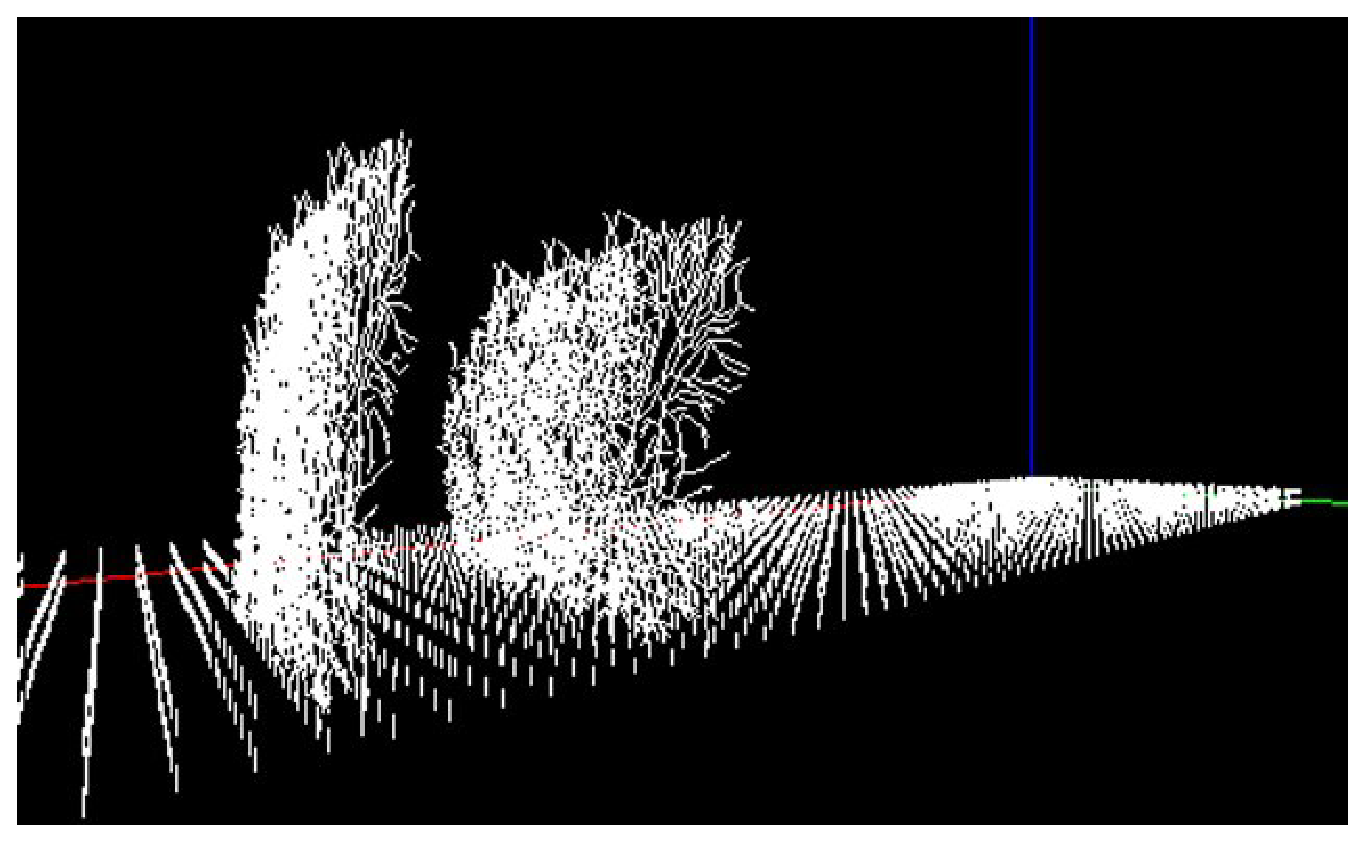
\includegraphics[scale=0.5]{figures/screenshot-1.eps}
\caption{{\bf Partial cerebellar cortex network :} 6 Purkinje and 6240 granule cells (330,000 equations).}
  \label{fig:pb-1}
\end{figure}

%\begin{figure}[h]
%  \centering
% 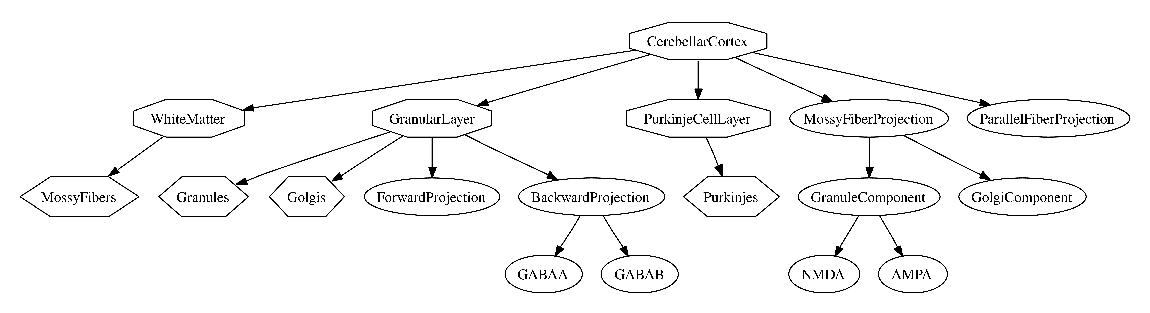
\includegraphics[scale=0.2]{figures/screenshot-2.eps}
% \caption{{\bf Model overview:} This overview is automatically generated by the Project Browser.}
%  \label{fig:pb-2}
%\end{figure}

\begin{figure}[h]
  \centering
 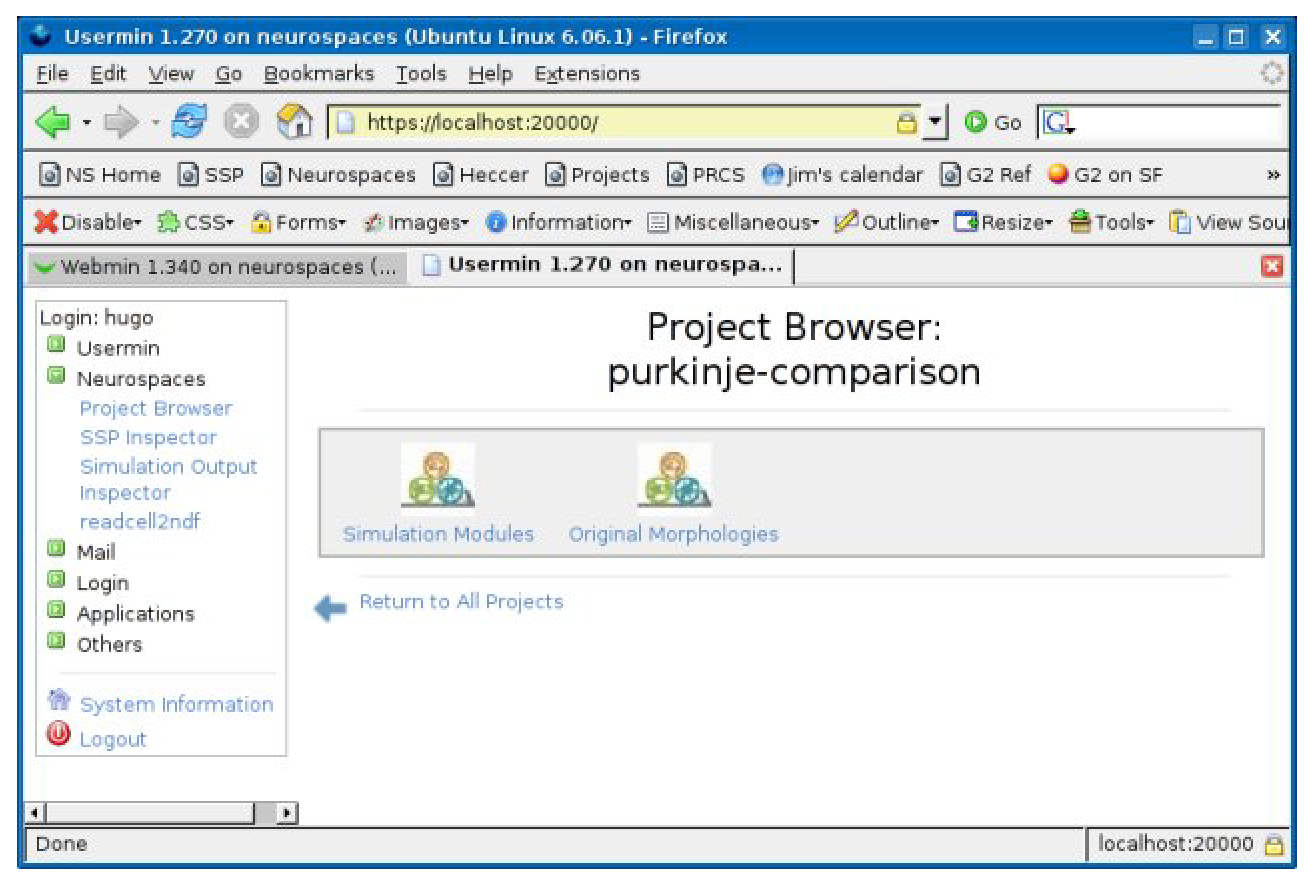
\includegraphics[scale=0.6]{figures/screenshot-3.eps}
 \caption{{\bf Screenshot of the Project Browser:} Purkinje cell comparative study.}
  \label{fig:pb-3}
\end{figure}

\begin{figure}[h]
  \centering
 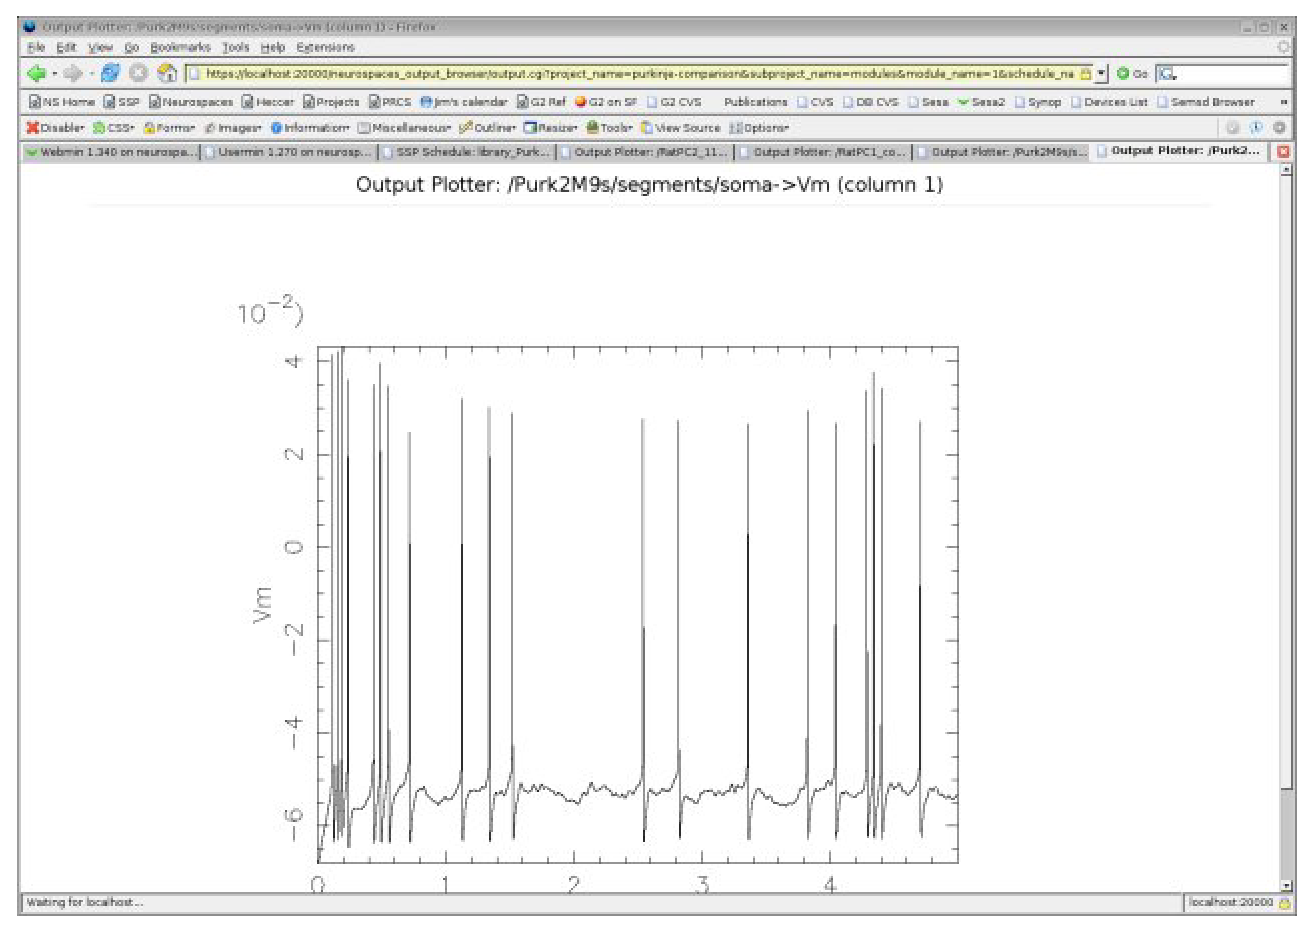
\includegraphics[scale=0.6]{figures/screenshot-4.eps}
 \caption{{\bf Project Browser output:} Purkinje cell soma membrane potential plot.}
  \label{fig:pb-4}
\end{figure}

%\begin{figure}[h]
%  \centering
% 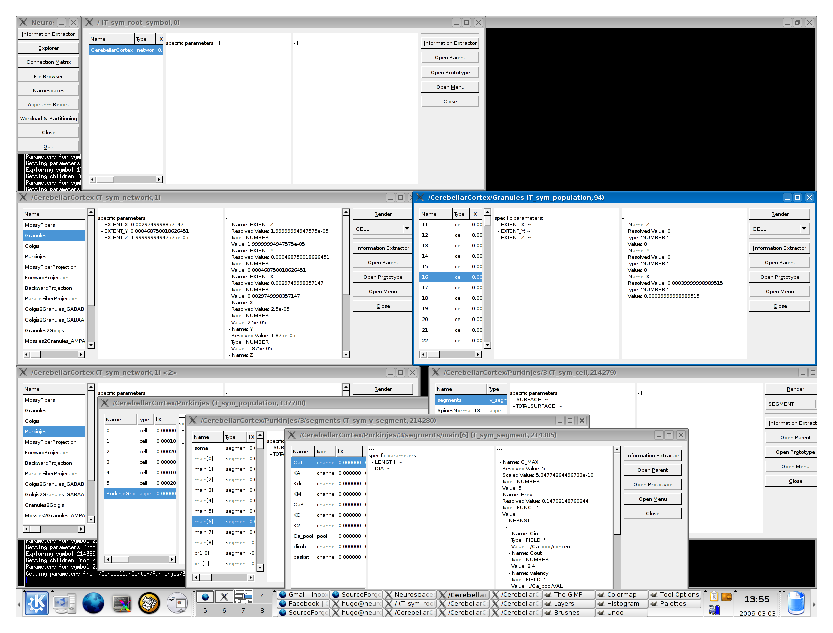
\includegraphics[scale=3.5]{figures/screenshot-5.eps}
%  \caption{{\bf Screenshot of the Project Browser:} Full featured biological model explorer.}
%  \label{fig:pb-5}
%\end{figure}

%\begin{figure}[h]
%  \centering
% 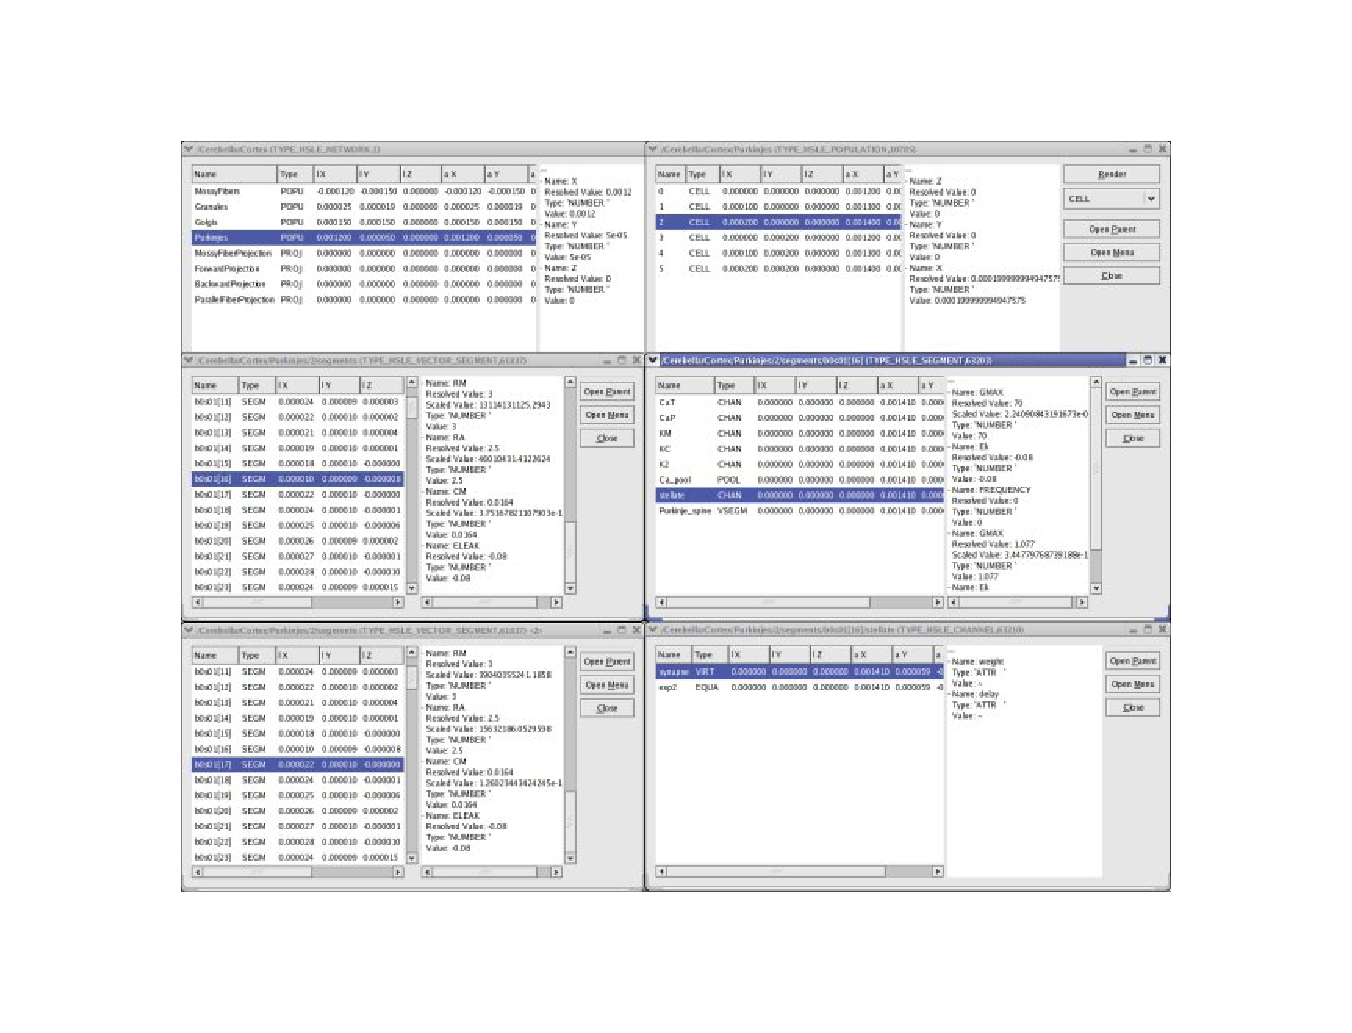
\includegraphics[scale=0.6]{figures/screenshot-6.eps}
%  \caption{{\bf Screenshot of the Project Browser}: Network connectivity matrix inspector--result set.}
%  \label{fig:pb-6}
%\end{figure}

\end{document}
